\chapter*{PlantaBot - Um Sistema Especialista para Supervisão e Manutenção de Planta Industrial}
\addcontentsline{toc}{chapter}{PlantaBot - Um Sistema Especialista para Supervisão e Manutenção de Planta Industrial}

\begin{flushright}
Sid Gubert
\end{flushright}

O PlantaBot é um assistente virtual especialista em supervisão e manutenção de uma planta industrial de pequeno porte. Seu objetivo é ajudar operadores e técnicos a interpretar as leituras de sensores, os alarmes e as ordens de serviço (OS) dos equipamentos.

Em uma planta instrumentada, uma leitura isolada de temperatura, pressão ou vibração raramente basta para decidir o que fazer \cite{mobley2002introduction}. Antes de agir, o técnico confere se a grandeza passou do limite operacional (\textit{setpoint}), a severidade dos alarmes ativos e se já há OS aberta para o equipamento. O PlantaBot reproduz esse raciocínio combinando um Grande Modelo de Linguagem (LLM) com uma base de conhecimento do domínio e com consultas aos dados da planta \cite{yang2025comprehensive,garridomerchan2026gofai}.

O mini-mundo adotado, ilustrado na Figura \ref{fig:minimundo-plantabot}, tem oito equipamentos em quatro setores (duas bombas, três compressores, dois motores e uma caldeira), cada um com faixas de operação para as grandezas monitoradas. Três serviços registram as leituras dos sensores, os alarmes e as OS de manutenção.

\begin{figure}[!ht]
\centering
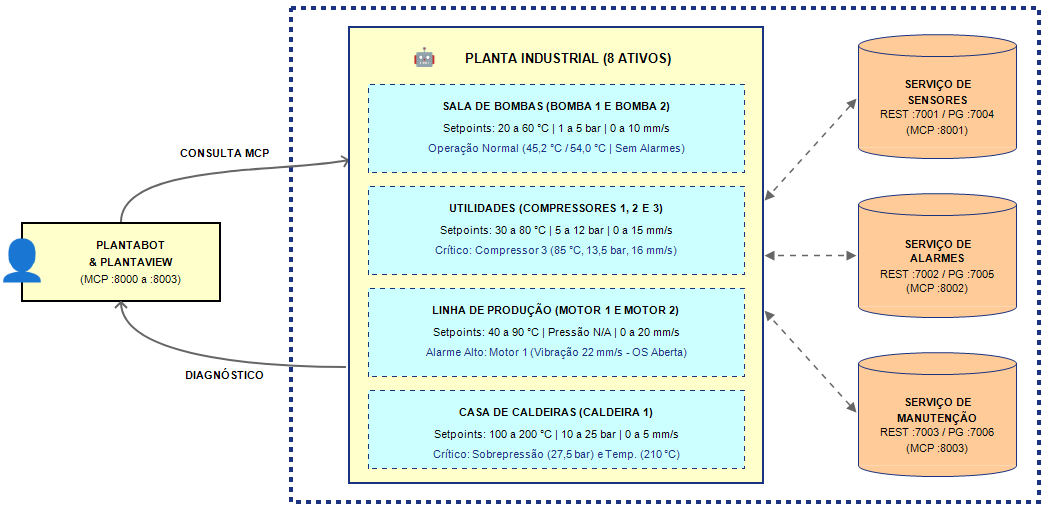
\includegraphics[width=0.7\textwidth]{capitulos/plantabot/minimundo.png}
\caption{Mini-mundo da planta industrial}
\label{fig:minimundo-plantabot}
\end{figure}

\section*{Arquitetura do PlantaBot}

A Figura \ref{fig:arquitetura-plantabot} exibe a arquitetura do PlantaBot. O usuário conversa com o especialista por um chat, no terminal ou na interface web, e cada pergunta vai para um LLM executado localmente pelo \textit{Ollama}. O \textit{prompt} dá ao modelo a persona de um perito em supervisão industrial, carrega a base de conhecimento (vinte pares de pergunta e resposta sobre os equipamentos, seus \textit{setpoints}, a classificação dos alarmes e os tipos de manutenção) e manda recusar perguntas fora do domínio.

A memória de trabalho reúne um cache semântico, que devolve a resposta já dada a uma pergunta de mesmo sentido, e o histórico das últimas mensagens da sessão, enviado ao LLM com cada nova pergunta.

\begin{figure}[!ht]
\centering
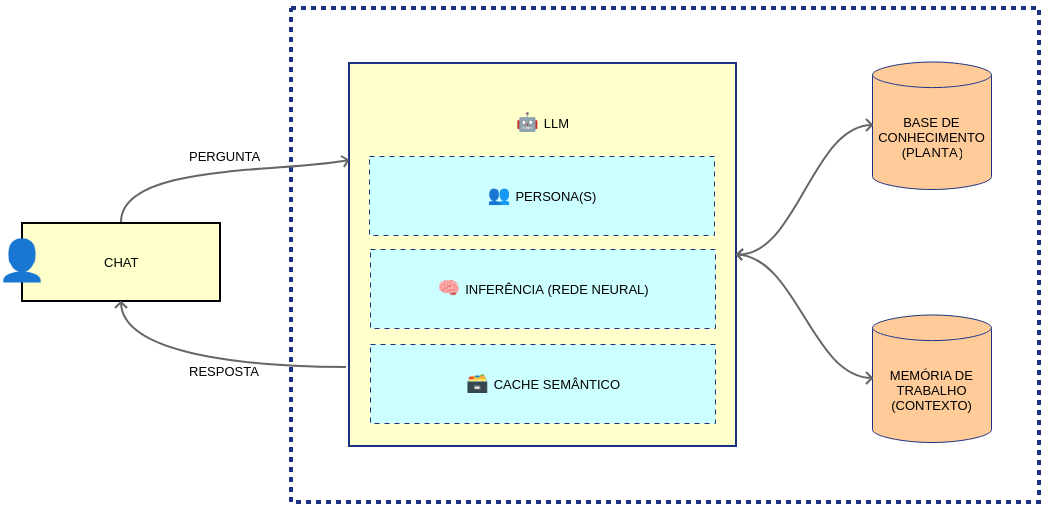
\includegraphics[width=0.8\textwidth]{capitulos/plantabot/arquitetura.png}
\caption{Arquitetura do PlantaBot}
\label{fig:arquitetura-plantabot}
\end{figure}

\section*{Ferramentas MCP}

A base de conhecimento diz como a planta deve operar, mas não qual é o seu estado atual. Para isso o PlantaBot usa ferramentas do \textit{Model Context Protocol} (MCP), protocolo que padroniza a descoberta e a chamada de recursos externos por aplicações com LLM \cite{mcp2026architecture}. Um único servidor MCP expõe dez ferramentas; ao iniciar, o chat se conecta a ele e repassa a lista ao modelo:

\begin{itemize}
    \item \textbf{Sensores:} \path{leituras_por_equipamento}, \path{leituras_por_grandeza} e \path{ultima_leitura} retornam as medições e os respectivos \textit{setpoints};
    \item \textbf{Alarmes:} \path{alarmes_por_equipamento}, \path{alarmes_por_severidade} e \path{resumo_alarmes} retornam os alarmes, sua severidade e seu estado;
    \item \textbf{Manutenção:} \path{ordens_por_equipamento}, \path{ordens_por_status} e \path{resumo_manutencao} retornam as OS e seu andamento;
    \item \textbf{Diagnóstico:} \path{diagnosticar_equipamento} reúne, em uma única chamada, os desvios de \textit{setpoint}, os alarmes ativos e as OS pendentes de um equipamento.
\end{itemize}

As ferramentas consultam os três serviços da planta, que são APIs REST com bancos de dados próprios. Se os serviços estiverem desligados, elas devolvem dados simulados, marcados no campo \texttt{fonte} do resultado, e o chat avisa o usuário.

\section*{Desenvolvimento e Avaliação}

O PlantaBot foi escrito em Python. A biblioteca \textit{openai} envia as mensagens ao \textit{Ollama}, que roda o modelo \texttt{qwen3:4b}. A \textit{sentence-transformers} gera o \textit{embedding} de cada pergunta e o \textit{chromadb} guarda esses vetores; a resposta sai do cache quando a distância de cosseno até uma pergunta anterior é de no máximo $0{,}20$. Recusas e respostas obtidas com ferramentas não entram no cache, pois estas dependem do estado da planta no momento. O servidor MCP usa o \texttt{FastMCP} e a interface web, o \textit{Chainlit}, que mostra a resposta enquanto é gerada, exibe cada ferramenta acionada como uma etapa expansível e plota as leituras dos sensores.

A Figura \ref{fig:funcionamento-plantabot} mostra uma sessão de uso na interface web. À esquerda, o pedido das leituras do Compressor 3 aciona uma ferramenta; com os serviços desligados, a interface avisa que os dados são simulados e mostra um gráfico com a faixa de operação e o valor lido de cada grandeza. À direita estão uma resposta gerada pelo LLM, a mesma resposta vinda do cache para uma pergunta reformulada e a recusa de uma pergunta fora do domínio.

\begin{figure}[!ht]
\centering
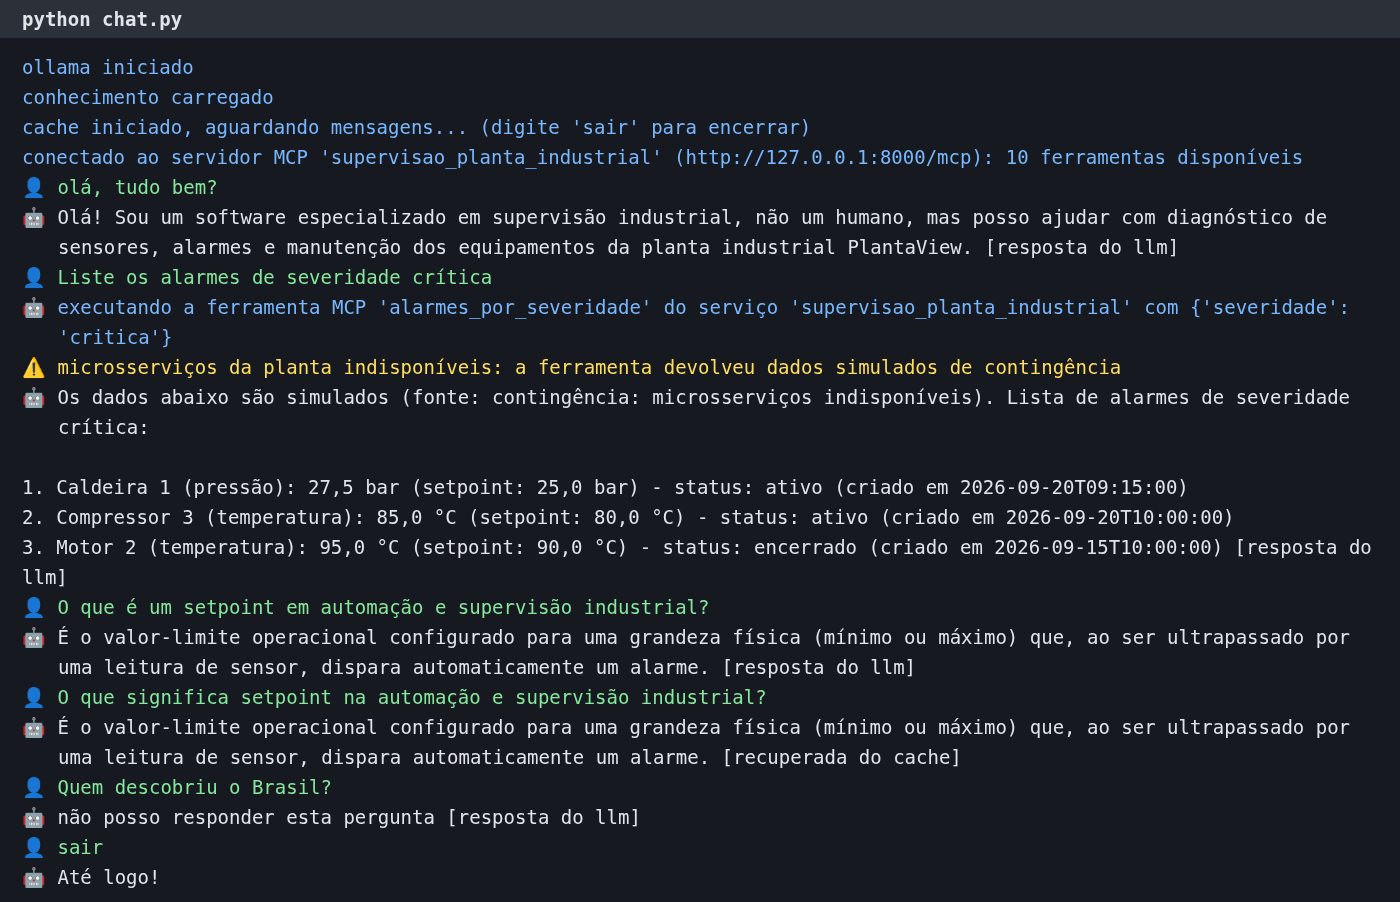
\includegraphics[width=0.8\textwidth]{capitulos/plantabot/funcionamento.png}
\caption{Funcionamento do PlantaBot na interface web}
\label{fig:funcionamento-plantabot}
\end{figure}

As respostas são avaliadas com a técnica \textit{LLM-as-a-Judge} \cite{azevedo2026julgamento}. O julgador é o \texttt{gemini-3.5-flash-lite}, do Google; usar um modelo de outro fornecedor evita que o assistente avalie a si próprio. Ele recebe, como instrução de sistema, sua persona e um gabarito com quatro perguntas da base de conhecimento. Antes de julgar o PlantaBot, o julgador analisa três respostas propositalmente erradas, para confirmar que sabe reprová-las. Na execução da Figura \ref{fig:julgamento-plantabot}, as três respostas erradas foram reprovadas e as quatro do assistente, aprovadas. Com uma amostra tão pequena, o teste confere o funcionamento do julgamento, mas não mede a acurácia do sistema.

\begin{figure}[!ht]
\centering
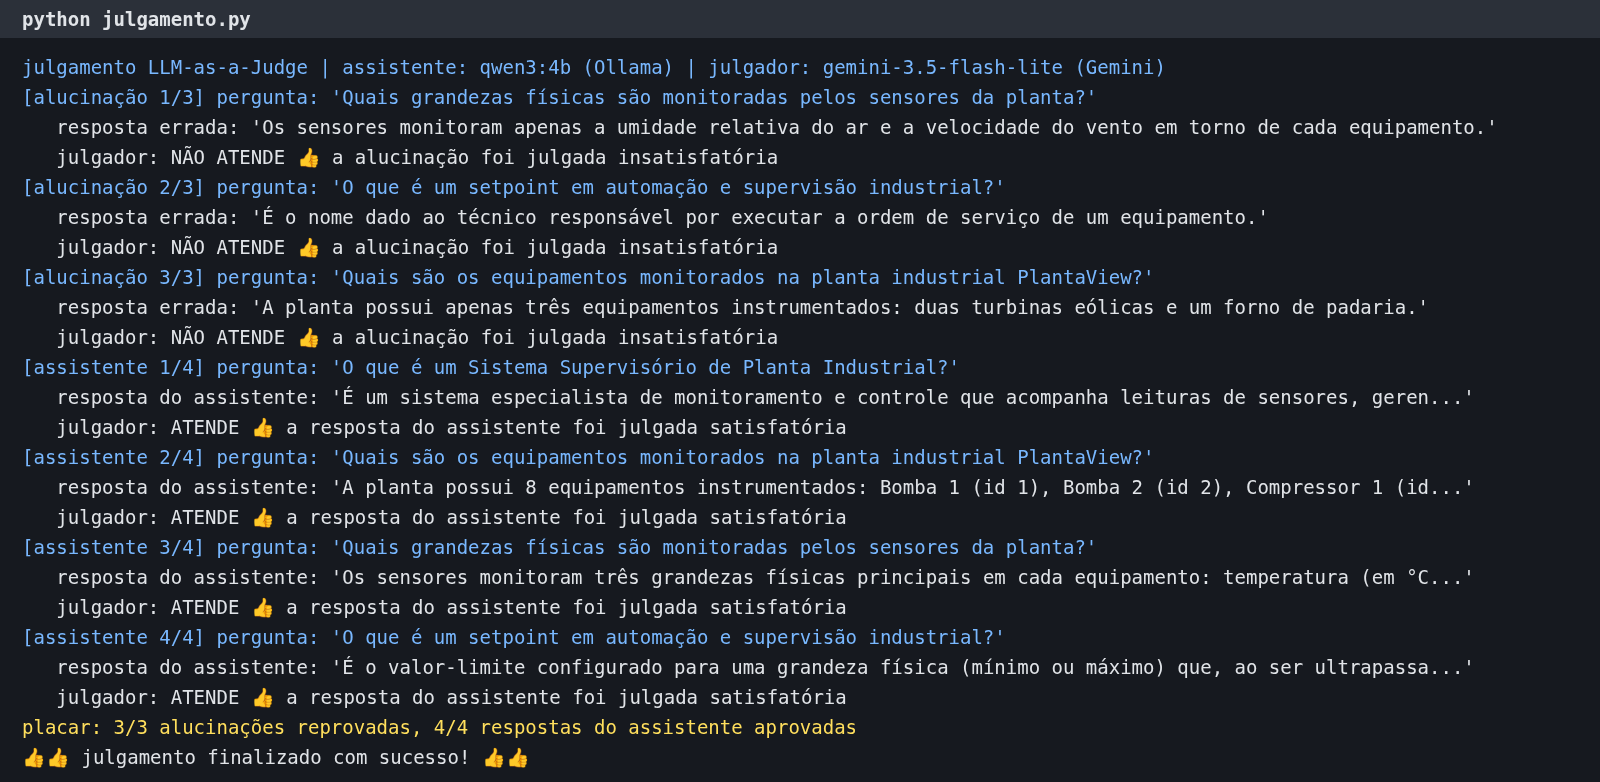
\includegraphics[width=1.0\textwidth]{capitulos/plantabot/julgamento.png}
\caption{Julgamento do PlantaBot}
\label{fig:julgamento-plantabot}
\end{figure}

\section*{Reproducibilidade e Reuso}

O código-fonte do PlantaBot pode ser consultado e (re)usado livremente através do link de acesso ao \href{https://github.com/sidgubert/supervisorio-especialista}{repositório do projeto}. Também se encontra disponibilizado no Zenodo um vídeo demonstrativo \href{https://zenodo.org/records/24356687}{neste link} (DOI \href{https://doi.org/10.5281/zenodo.24356687}{10.5281/zenodo.24356687}).
